\subsection{PIC}

The Particle-In-Cell (PIC) method uses both particles and grids for fluid simulation. Each simulation step involves five primary phases:

\begin{enumerate}
\item \textbf{Transfer to Grid}: Particle velocities are transferred to nearby grid cells using B-spline weighting functions.
The compact quadratic B-spline kernel used is:
\begin{equation}
w(r) =
\begin{cases}
0.75 - r^2, & 0 \le r < 0.5 \\
0.5 \cdot (1.5 - r)^2, & 0.5 \le r < 1.5 \\
0, & \text{otherwise}
\end{cases}
\end{equation}

\item \textbf{Apply Gravity}: Gravity force is applied directly to vertical grid velocities.
Grid velocity is updated using:
\begin{equation}
\vec{v}_{i,j}.y \mathrel{-}= g \cdot \Delta t
\end{equation}

\item \textbf{Solve Pressure}: The pressure Poisson equation is solved using Jacobi iteration. Initially, divergence is calculated for each grid cell. 
\begin{equation}
  \nabla \cdot \vec{v}_{i,j} = \frac{v_{i+1,j}.x - v_{i-1,j}.x}{2} + \frac{v_{i,j+1}.y - v_{i,j-1}.y}{2}
  \end{equation}

Then, pressure values are iteratively adjusted to minimize divergence, enforcing incompressibility.
\begin{equation}
  p_{i,j}^{(k+1)} = \frac{1}{N} \left( \sum_{\text{fluid neighbors}} p^{(k)} - \nabla \cdot \vec{v}_{i,j} \right)
  \end{equation}
  where \( N \) is the number of neighboring fluid cells.

The velocity field is updated by subtracting the pressure gradient.
\begin{equation}
  \vec{v}_{i,j}.x \mathrel{-}= \frac{p_{i+1,j} - p_{i-1,j}}{2}, \quad
  \vec{v}_{i,j}.y \mathrel{-}= \frac{p_{i,j+1} - p_{i,j-1}}{2}
  \end{equation}

\item \textbf{Transfer Back to Particles}: Updated grid velocities are interpolated back onto particles.
\begin{equation}
  \vec{v}_p = \sum_{(i,j)} w_{(i,j) \rightarrow p} \cdot \vec{v}_{i,j}
  \end{equation}

\item \textbf{Move Particles}: Particles are advected according to their updated velocities. Boundary conditions are enforced by repositioning particles inside the domain and setting boundary normal velocities to zero.
\begin{equation}
  \vec{x}_p \mathrel{+}= \vec{v}_p \cdot \Delta t
  \end{equation}
\end{enumerate}

\subsubsection{Intermediate Results and Diagrams (PIC)}

In the following figures, the \textbf{yellow arrows} show the grid velocity at some grid points.

\begin{figure}[h]
    \centering
    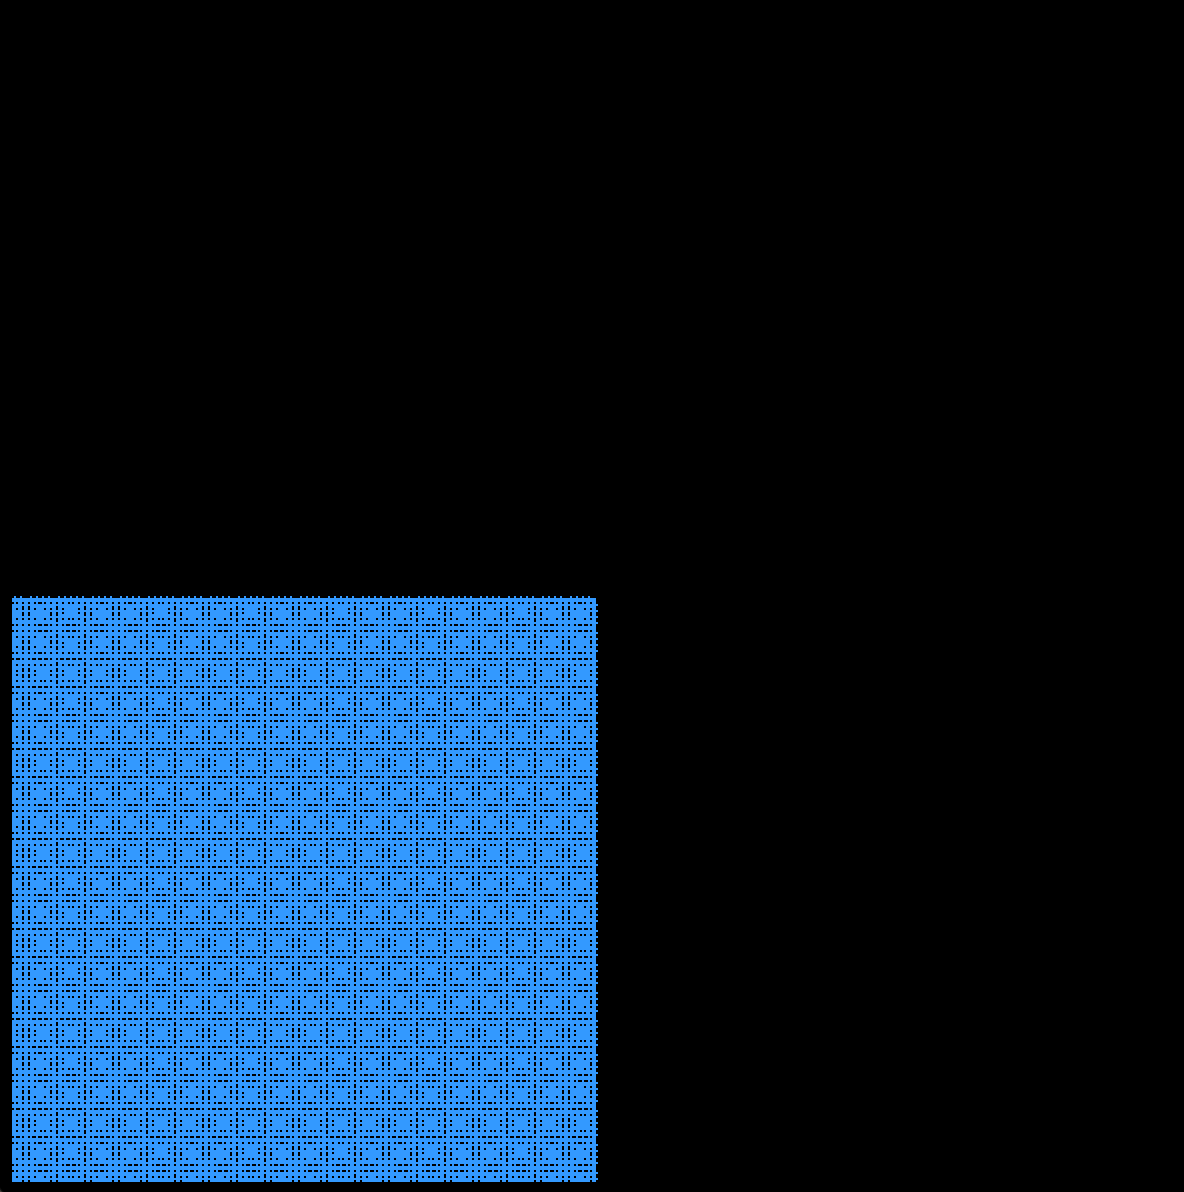
\includegraphics[width=0.25\textwidth]{figures/pic_init.png}
    \caption{Initially, all particles are in the bottom-left corner.}
    \label{fig:pic_init}
\end{figure}

\begin{figure}[h]
    \centering
    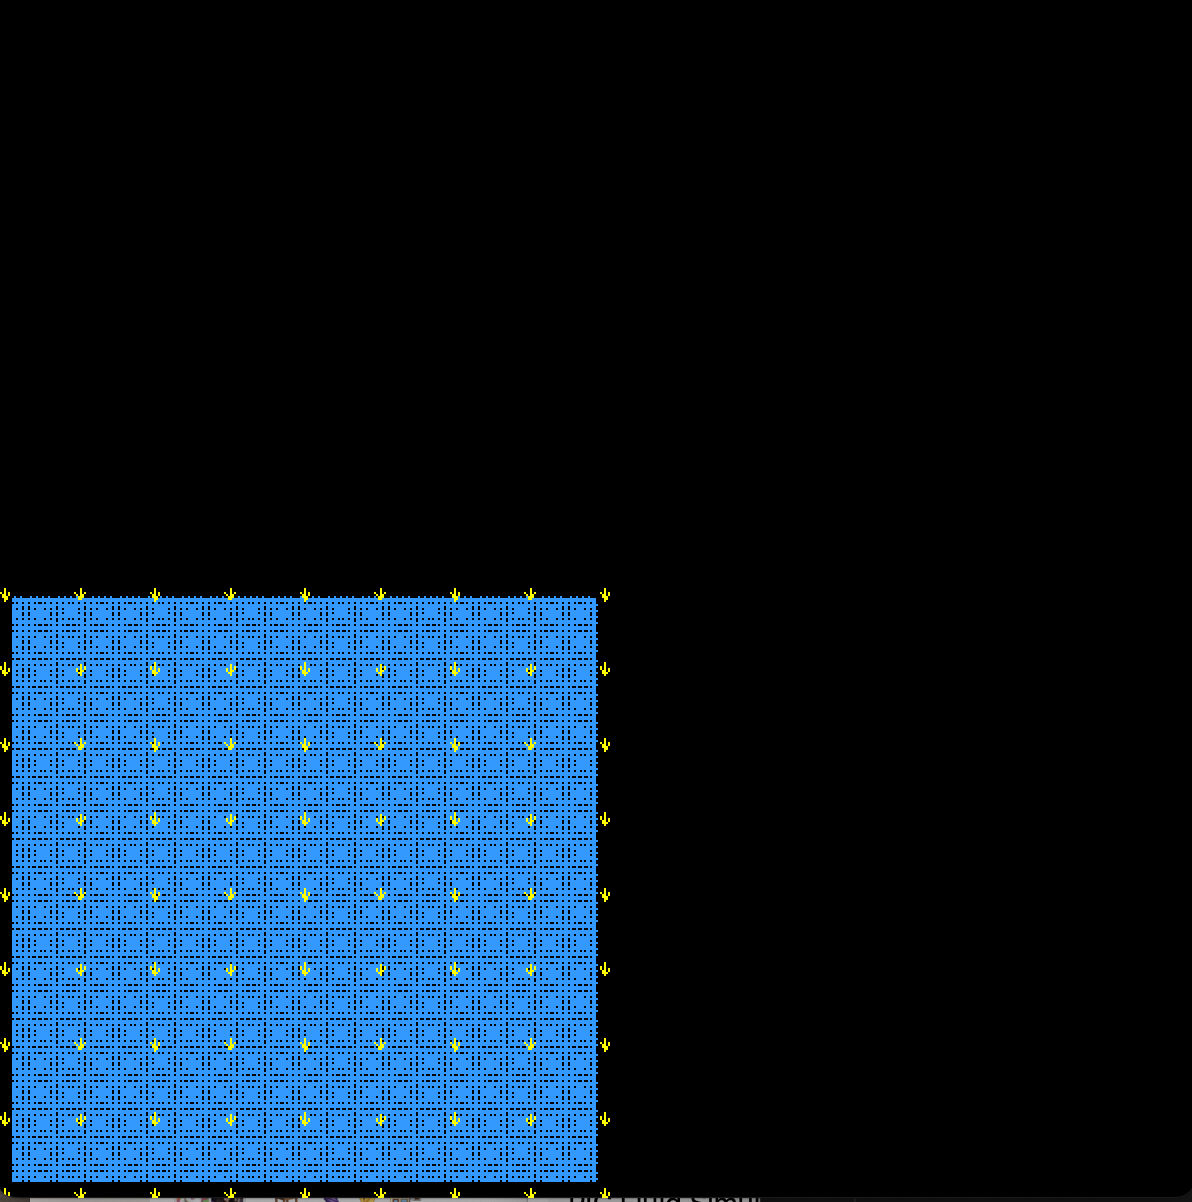
\includegraphics[width=0.25\textwidth]{figures/pic_apply_g.png}
    \caption{After gravity is added, the grid velocity points downward.}
    \label{fig:pic_gravity}
\end{figure}

\begin{figure}[h]
    \centering
    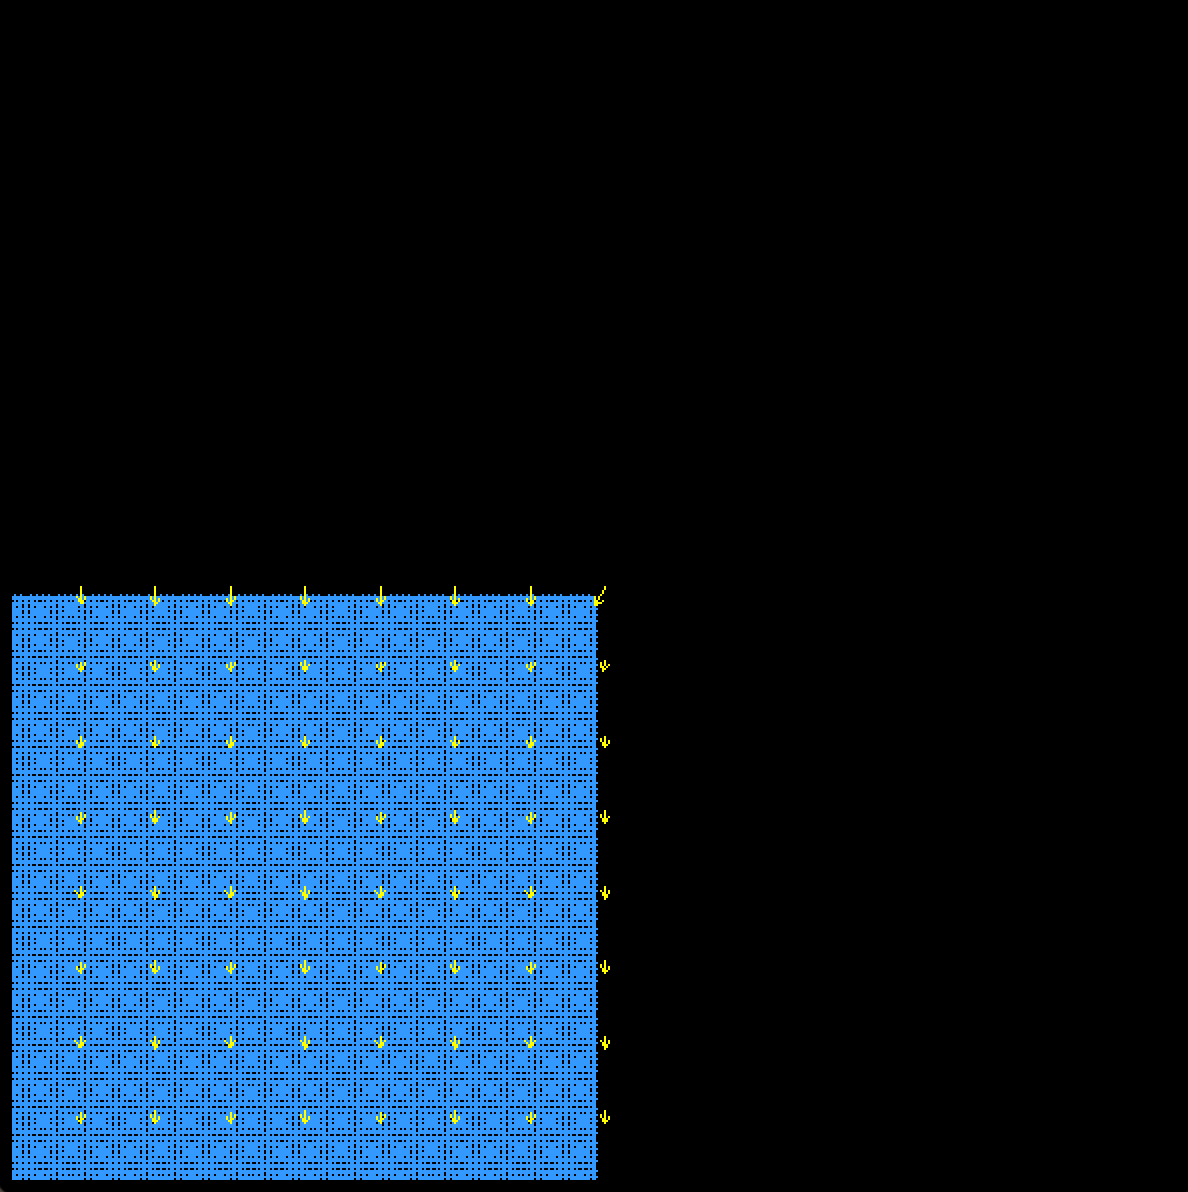
\includegraphics[width=0.25\textwidth]{figures/pic_solve_pr.png}
    \caption{After solving pressure, the grid velocity becomes balanced.}
    \label{fig:pic_pressure}
\end{figure}

\begin{figure}[h]
    \centering
    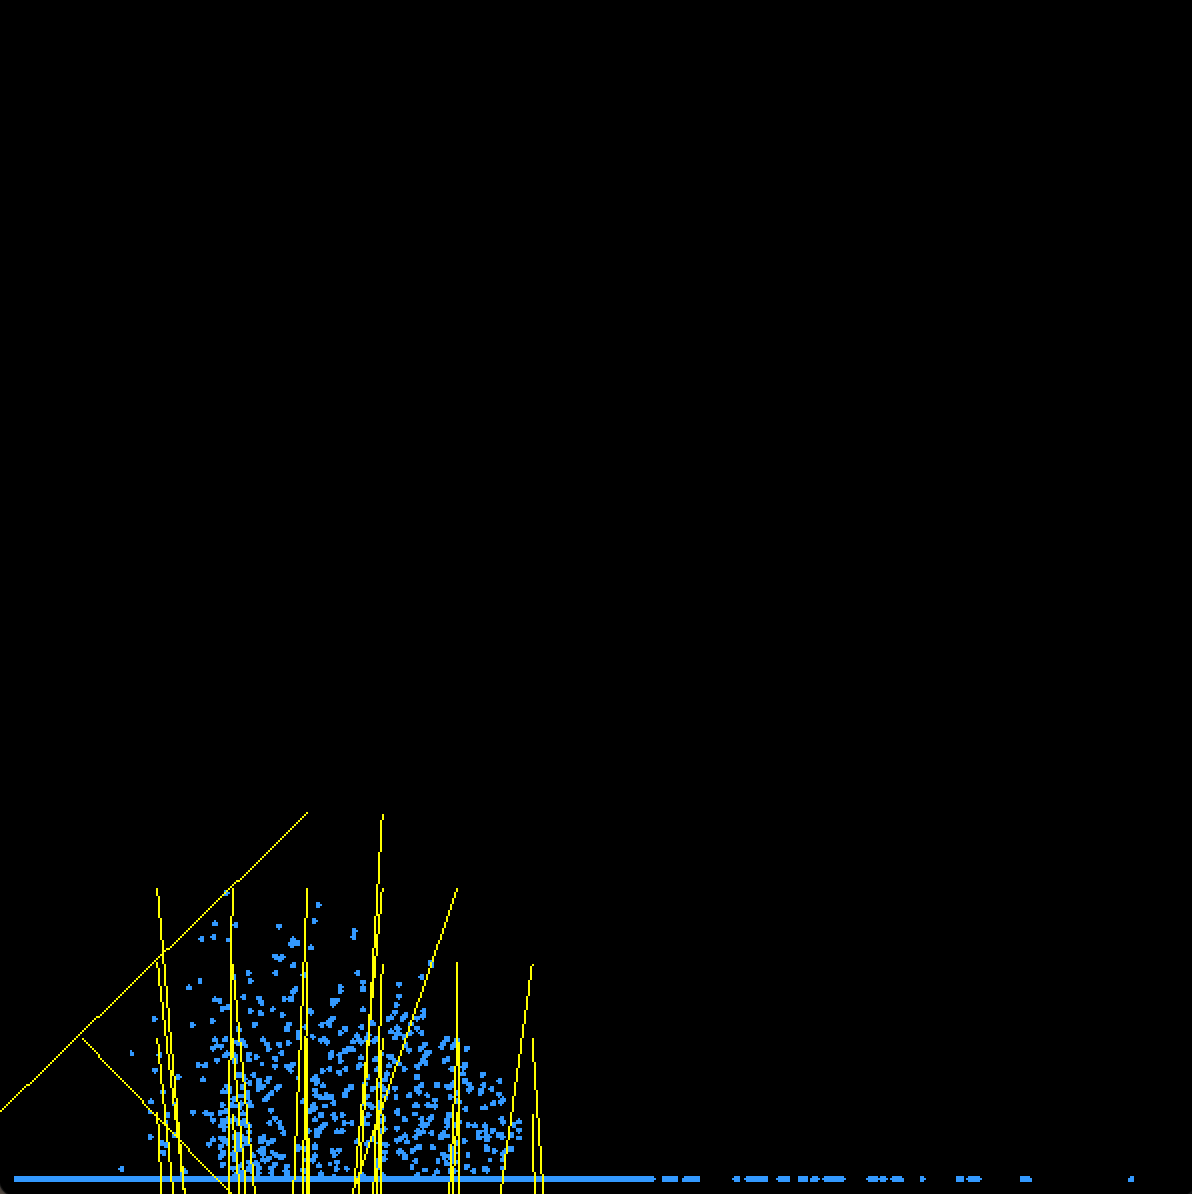
\includegraphics[width=0.25\textwidth]{figures/pic_interm.png}
    \caption{Particles start to move after updating their velocity.}
    \label{fig:pic_inter}
\end{figure}

\subsection{PIC/FLIP Implementation}

The PIC/FLIP hybrid method follows a similar pipeline but differs in how particle velocities are updated:

\begin{enumerate}
\item Before applying gravity, the current grid velocity is stored.

\item After solving the pressure, the difference between the new and old grid velocities is computed.

\item Particle velocities are updated using a blend of PIC and FLIP:
\begin{equation}
  \begin{aligned}
  &\text{blended\_velocity} \\
  &= \text{ particle\_velocity} \\
  &+ \text{ flip\_ratio} \cdot (\text{new\_grid\_velocity} - \text{old\_grid\_velocity})
  \end{aligned}
\end{equation}
where a flip\_ratio of 0 corresponds to pure PIC, and values approaching 1 resemble FLIP.

\item Particles are then advected in the same manner as the PIC method, including boundary handling.
\end{enumerate}

\subsubsection{Intermediate Results and Diagrams (PIC/FLIP)}
\begin{figure}[h]
  \centering
  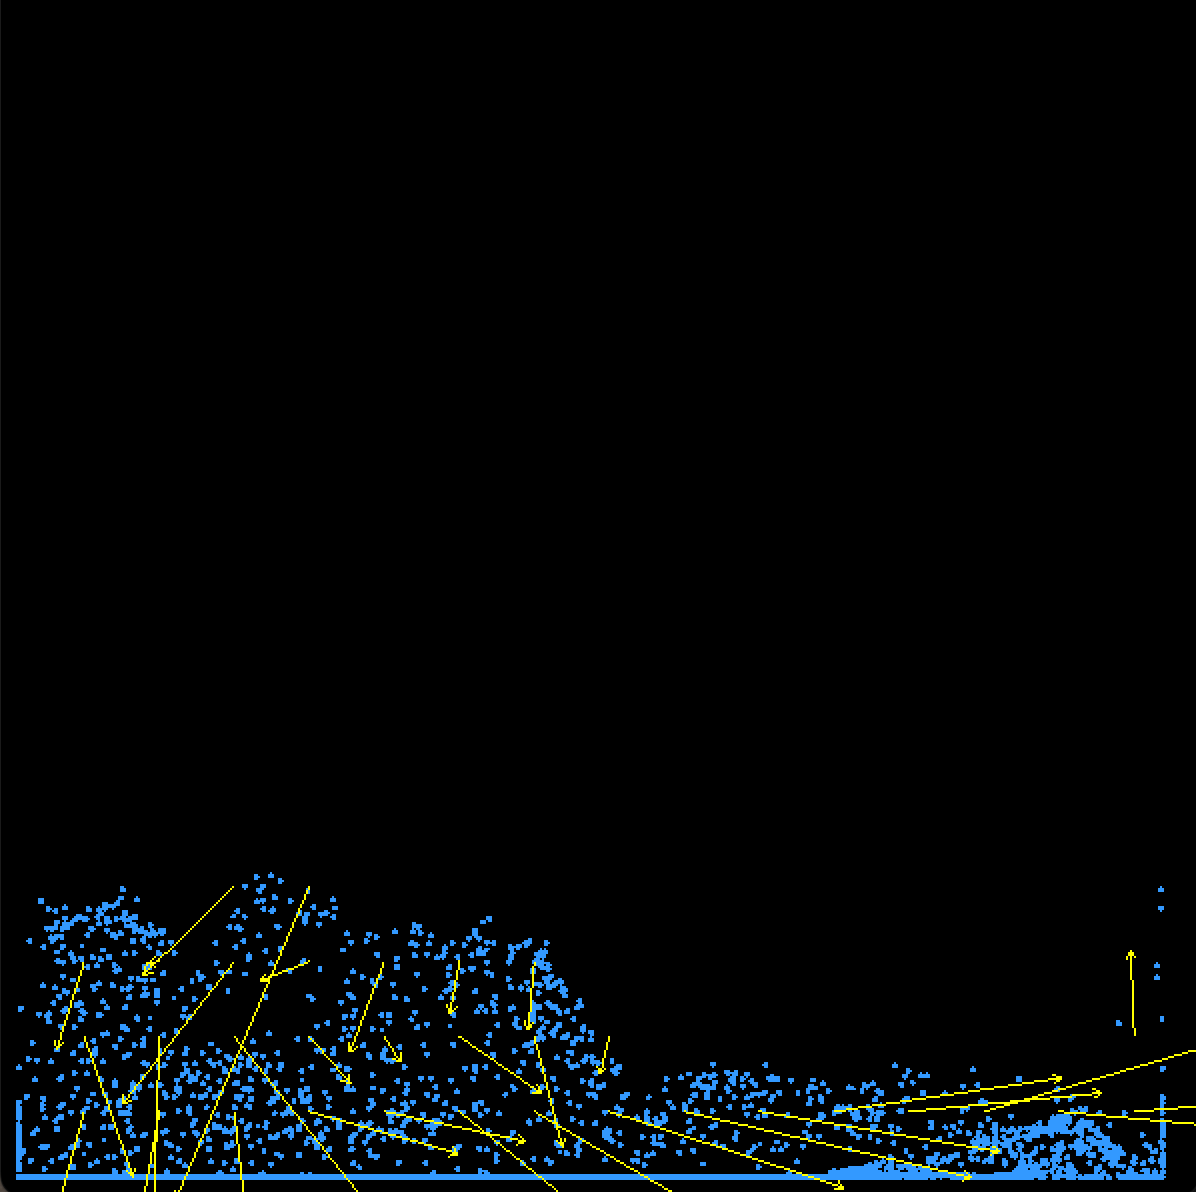
\includegraphics[width=0.25\textwidth]{figures/pic_flip_interm.png}
  \caption{With PIC/FLIP, the motion is more dynamic than pure PIC.}
  \label{fig:pic_flip}
\end{figure}

